\documentclass[12pt]{article}\usepackage[]{graphicx}\usepackage[]{color}
% maxwidth is the original width if it is less than linewidth
% otherwise use linewidth (to make sure the graphics do not exceed the margin)
\makeatletter
\def\maxwidth{ %
  \ifdim\Gin@nat@width>\linewidth
    \linewidth
  \else
    \Gin@nat@width
  \fi
}
\makeatother

\definecolor{fgcolor}{rgb}{0.345, 0.345, 0.345}
\newcommand{\hlnum}[1]{\textcolor[rgb]{0.686,0.059,0.569}{#1}}%
\newcommand{\hlstr}[1]{\textcolor[rgb]{0.192,0.494,0.8}{#1}}%
\newcommand{\hlcom}[1]{\textcolor[rgb]{0.678,0.584,0.686}{\textit{#1}}}%
\newcommand{\hlopt}[1]{\textcolor[rgb]{0,0,0}{#1}}%
\newcommand{\hlstd}[1]{\textcolor[rgb]{0.345,0.345,0.345}{#1}}%
\newcommand{\hlkwa}[1]{\textcolor[rgb]{0.161,0.373,0.58}{\textbf{#1}}}%
\newcommand{\hlkwb}[1]{\textcolor[rgb]{0.69,0.353,0.396}{#1}}%
\newcommand{\hlkwc}[1]{\textcolor[rgb]{0.333,0.667,0.333}{#1}}%
\newcommand{\hlkwd}[1]{\textcolor[rgb]{0.737,0.353,0.396}{\textbf{#1}}}%
\let\hlipl\hlkwb

\usepackage{framed}
\makeatletter
\newenvironment{kframe}{%
 \def\at@end@of@kframe{}%
 \ifinner\ifhmode%
  \def\at@end@of@kframe{\end{minipage}}%
  \begin{minipage}{\columnwidth}%
 \fi\fi%
 \def\FrameCommand##1{\hskip\@totalleftmargin \hskip-\fboxsep
 \colorbox{shadecolor}{##1}\hskip-\fboxsep
     % There is no \\@totalrightmargin, so:
     \hskip-\linewidth \hskip-\@totalleftmargin \hskip\columnwidth}%
 \MakeFramed {\advance\hsize-\width
   \@totalleftmargin\z@ \linewidth\hsize
   \@setminipage}}%
 {\par\unskip\endMakeFramed%
 \at@end@of@kframe}
\makeatother

\definecolor{shadecolor}{rgb}{.97, .97, .97}
\definecolor{messagecolor}{rgb}{0, 0, 0}
\definecolor{warningcolor}{rgb}{1, 0, 1}
\definecolor{errorcolor}{rgb}{1, 0, 0}
\newenvironment{knitrout}{}{} % an empty environment to be redefined in TeX

\usepackage{alltt}
\usepackage{amsmath,amssymb,mathrsfs,fancyhdr,syntonly,lastpage,hyperref,enumitem,graphicx,subcaption, tikz, caption, float}
\usepackage[authoryear]{natbib} % Natbib options, [numbers] would give numerical citations.
\bibpunct{(}{)}{;}{a}{,}{,} % Tells it how you want references displaying in the text.

\usepackage[thmmarks,thref]{ntheorem}

\theoremstyle{nonumberplain}
\theoremheaderfont{\itshape}
\theorembodyfont{\upshape}
\theoremseparator{.}
\theoremsymbol{\ensuremath{\square}}
\newtheorem{solution}{Solution}

\hypersetup{colorlinks=true,urlcolor=black}

\usepackage{xcolor}

\newcommand{\hh}[1]{{\color{orange}{#1}}}

\topmargin      -1.5cm   % read Lamport p.163
\oddsidemargin  -0.04cm  % read Lamport p.163
\evensidemargin -0.04cm  % same as oddsidemargin but for left-hand pages
\textwidth      16.59cm
\textheight     23.94cm
\parskip         7.2pt   % sets spacing between paragraphs
\parindent         0pt   % sets leading space for paragraphs
\pagestyle{empty}        % Uncomment if don't want page numbers
\pagestyle{fancyplain}
\author{Charlotte Roiger}
\title{Hough Transforms for Groove Identification in Land Engraved Areas (LEAs) on Fired Bullets}


\IfFileExists{upquote.sty}{\usepackage{upquote}}{}
\begin{document}
\lhead{\today}
\chead{CSAFE - Hough Grooves Document Process}
\rhead{Page \thepage\ of \pageref{LastPage}}

\begin{titlepage}
   \begin{center}
       \vspace*{1cm}

       \textbf{Hough Transforms for Groove Identification in Land Engraved Areas (LEAs) on Fired Bullets}

            
       \vspace{1 cm}

       \textbf{Charlotte Roiger}

       \vskip 1in
            
       A thesis submitted to the graduate faculty \\
       in partial fulfillment of the requirements for the degree of\\
       MASTER OF SCIENCE
            
       \vspace{0.8cm}
       
       Major: Statistics
       \vspace{2cm}
       Program of Study Committee:\\
       Heike Hofmann, Major Professor \\
       Jennifer Newman \\
       Yumou Qiu
       
       \vspace{0.8cm}
       The student author, whose presentation of the scholarship herein was approved by the program
of study committee, is solely responsible for the content of this thesis. The Graduate College will
ensure this thesis is globally accessible and will not permit alterations after a degree is conferred.
     \vspace{3cm}
            
       Iowa State University\\
       Ames, Iowa\\
       2020\\
       Copyright \textcopyright Charlotte Roiger, 2020. All Rights Reserved.
            
   \end{center}
\end{titlepage}

\section{Introduction}

When firearms and toolmark examiners (FTEs) try to match fired bullets they use a form of visual inspection to determine whether two bullets were fired from the same gun. When a bullet is  fired, manufacturing imperfections in the rifling of the barrel of the gun  leave marks, thought to be a unique to a barrel. Firearms examiners utilize these marks to make identifications by matching striation patterns between bullets. A 2005 court case known as \textit{United States vs. Green}, established that firearms examiners cannot conclude that a specific bullet was fired from a specific gun ``to the exclusion of every other firearm in the world". That in fact the conclusion of a definitive match stretches beyond the data and methodology available to firearms examiners at the time.  Similarly, in 2009 the National Academy of Sciences published a report that criticized the scientific validity of forensic firearms identification and many other forensic methods. Both of these reports highlight the need for objective quantitative assessments of firearms identification. 

As three dimensional scanning techniques have improved, new ways of bullet identification are being developed that rely on  statistical and machine learning methodology to automate bullet identification. One such example of automated bullet matching can be found in \cite{hare2017}, where the authors created an algorithm  that provides a probabilistic assessment of the strength of a match between two bullets. A key component of the algorithm  is the identification of ``shoulder locations" of bullet lands to improve the extraction of bullet signatures. In Figure \ref{fig:hare-bullet-anatomy-image} from \cite{hare2017} we see an example of a digital rendering of a bullet land, showing the top and side profiles respectively. The raised portions of the bullet land profile shown in Figure 1a are the shoulder locations in question and are the places where the bullet does not come in contact with the rifling of the gun barrel. 



\begin{knitrout}
\definecolor{shadecolor}{rgb}{0.969, 0.969, 0.969}\color{fgcolor}\begin{figure}[H]

{\centering 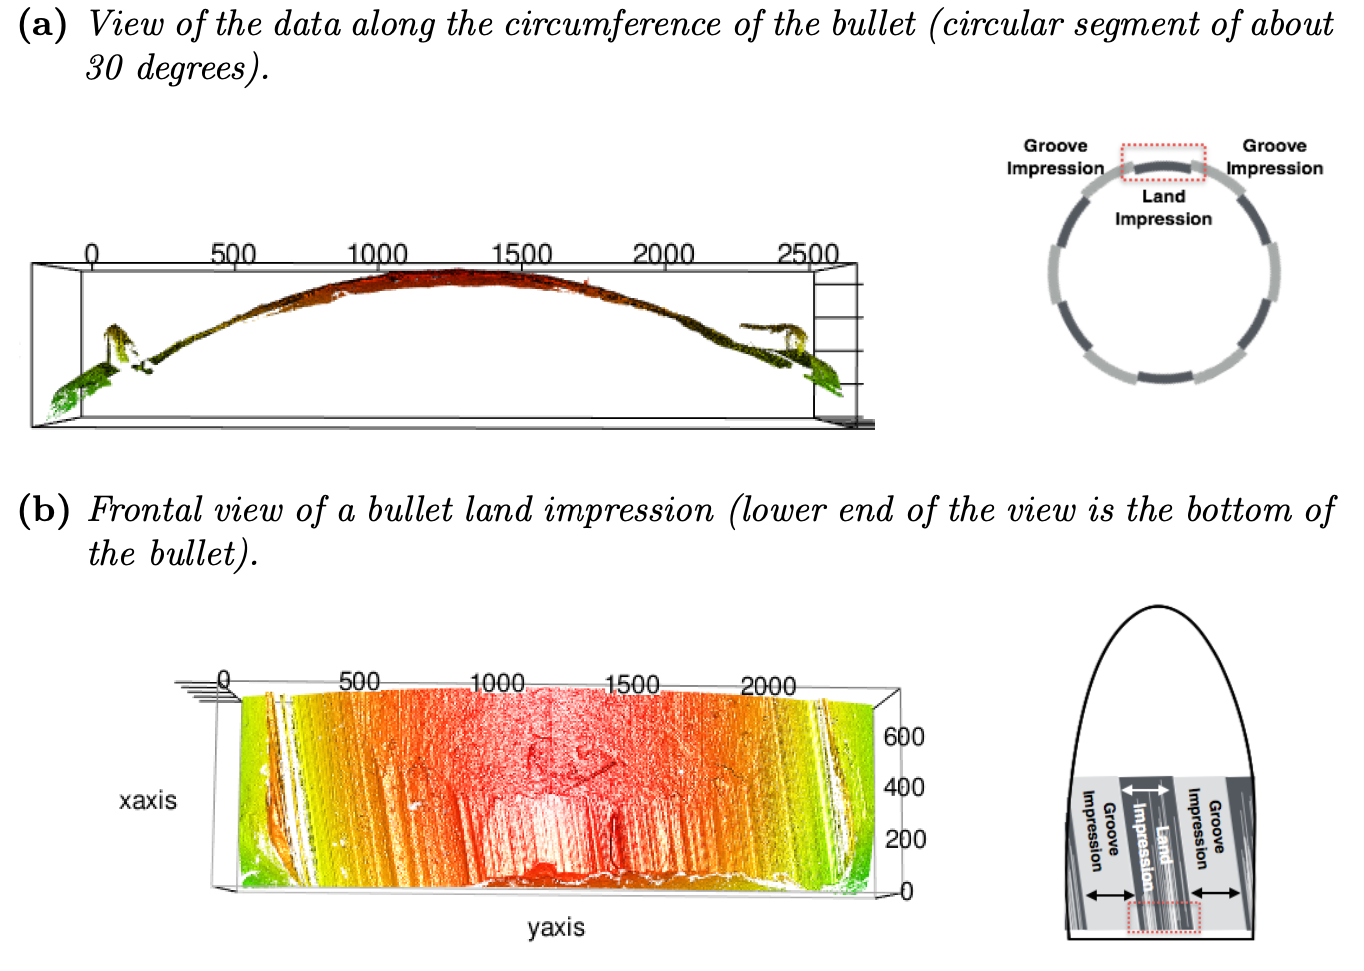
\includegraphics[width=0.5\linewidth]{../images/hare-bullet-anatomy-image} 

}

\caption[Example of a groove-to-groove scan of a bullet land impression]{Example of a groove-to-groove scan of a bullet land impression. The red-dotted rectangle on the right shows the location and orientation of the segment}\label{fig:hare-bullet-anatomy-image}
\end{figure}


\end{knitrout}


\begin{knitrout}
\definecolor{shadecolor}{rgb}{0.969, 0.969, 0.969}\color{fgcolor}\begin{figure}[H]

{\centering 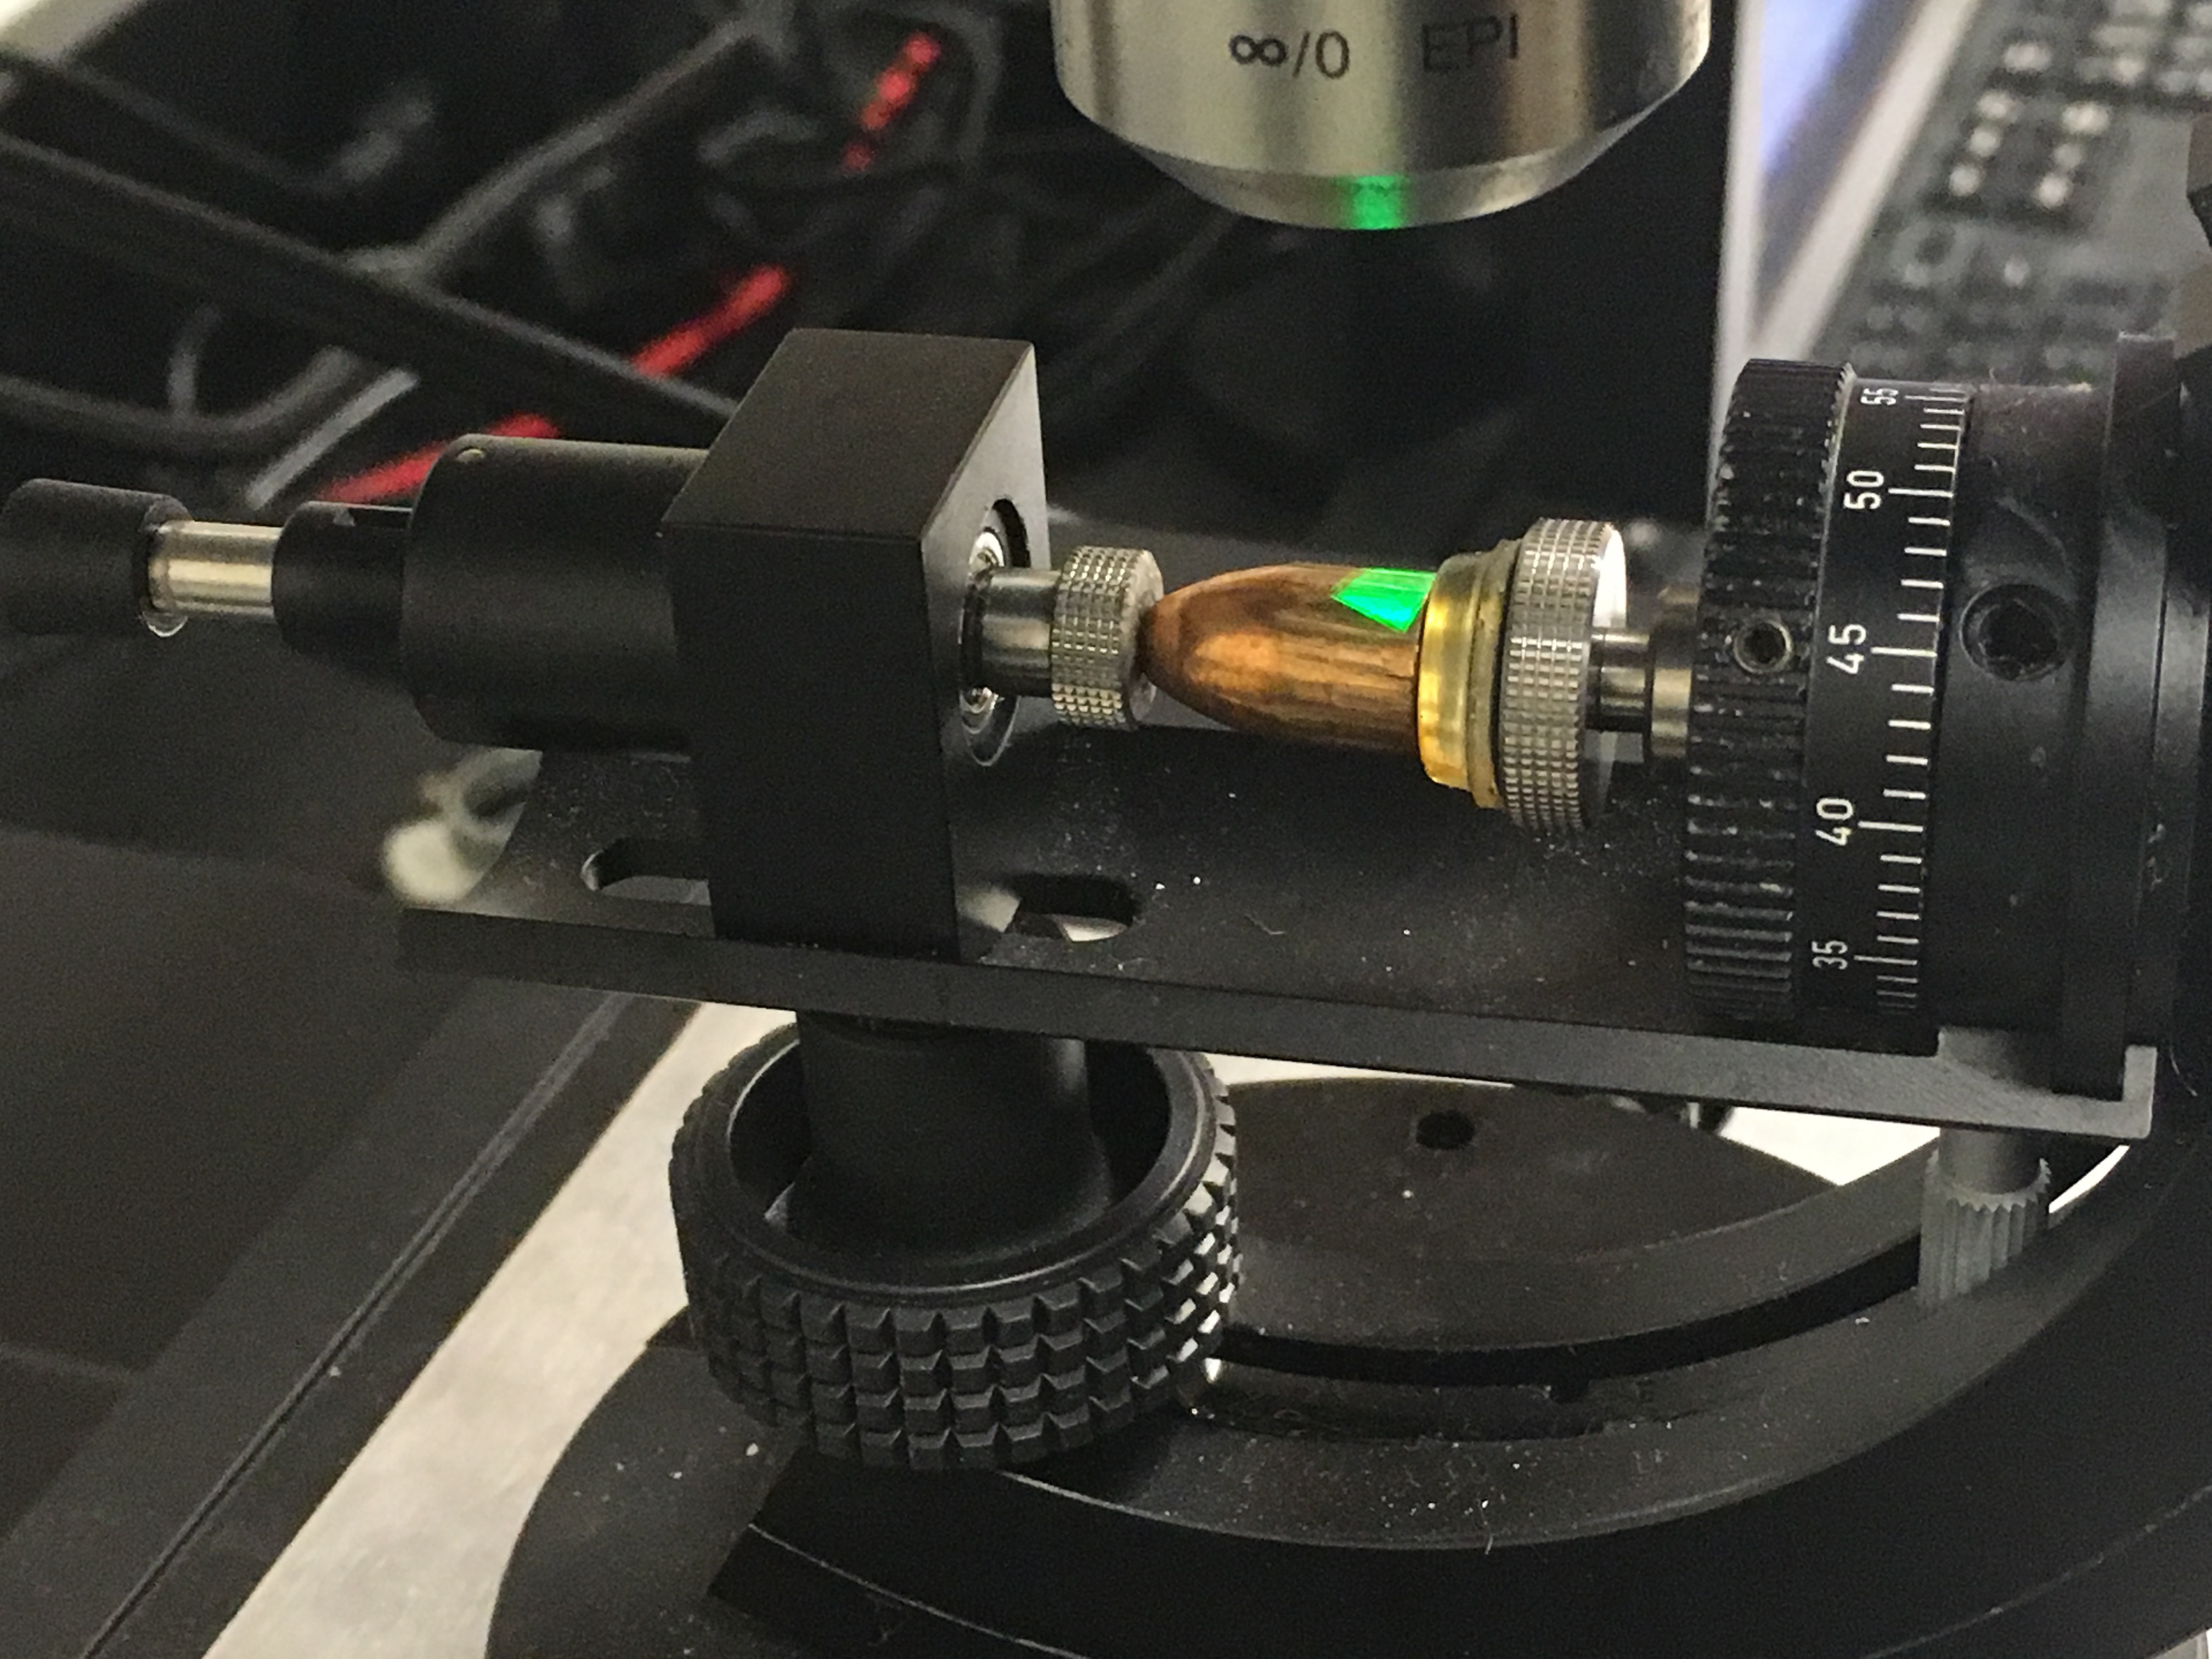
\includegraphics[width=0.5\linewidth]{../images/microscope-bullet} 

}

\caption[Bullet in a stage under a confocal light microscope]{Bullet in a stage under a confocal light microscope. The green lit area covers the scan of a LEA (land engraved area).}\label{fig:microscope-bullet}
\end{figure}


\end{knitrout}

Figure \ref{fig:microscope-bullet} demonstrates how three dimensional scans are taken using a Confocal light microscope. These scans then result in a three dimensional image as shown in Figure \ref{fig:crosscut-location-example}. The Data from these high-resolution scans is stored in the form of scans called ``x3p"(XML 3-D Surface Profile). Each scan consists of height measurements collected over an $x$-$y$ grid, which can be rendered similar to a grey-scale image. To read-in and manipulate the x3p files we utilize the package `x3ptools` to orient or transform the scans as needed for image processing. However, for use in statistical analyses these three-dimensional scans are  turned into a two-dimensional visualization of a single crosscut from a bullet land as shown in Figure \ref{fig:crosscut-motivation}. Figure \ref{fig:crosscut-location-example} shows the location of the crosscut on the three dimensional bullet scan, where crosscuts are chosen using the x3p\_crosscut\_optimize function from the x3ptools package. 

\begin{knitrout}
\definecolor{shadecolor}{rgb}{0.969, 0.969, 0.969}\color{fgcolor}\begin{figure}[H]

{\centering 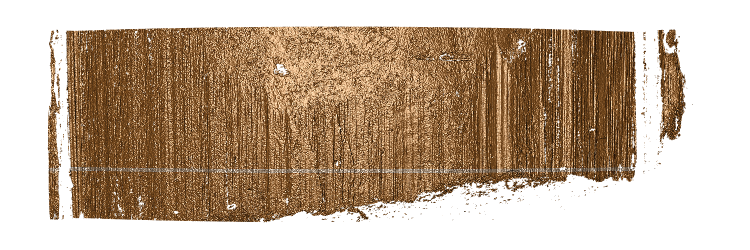
\includegraphics[width=\maxwidth]{../images/crosscut-location-example} 

}

\caption[Optimized crosscut location shown as a grey line along bullet profile]{Optimized crosscut location shown as a grey line along bullet profile}\label{fig:crosscut-location-example}
\end{figure}


\end{knitrout}



\begin{knitrout}
\definecolor{shadecolor}{rgb}{0.969, 0.969, 0.969}\color{fgcolor}\begin{figure}[H]

{\centering 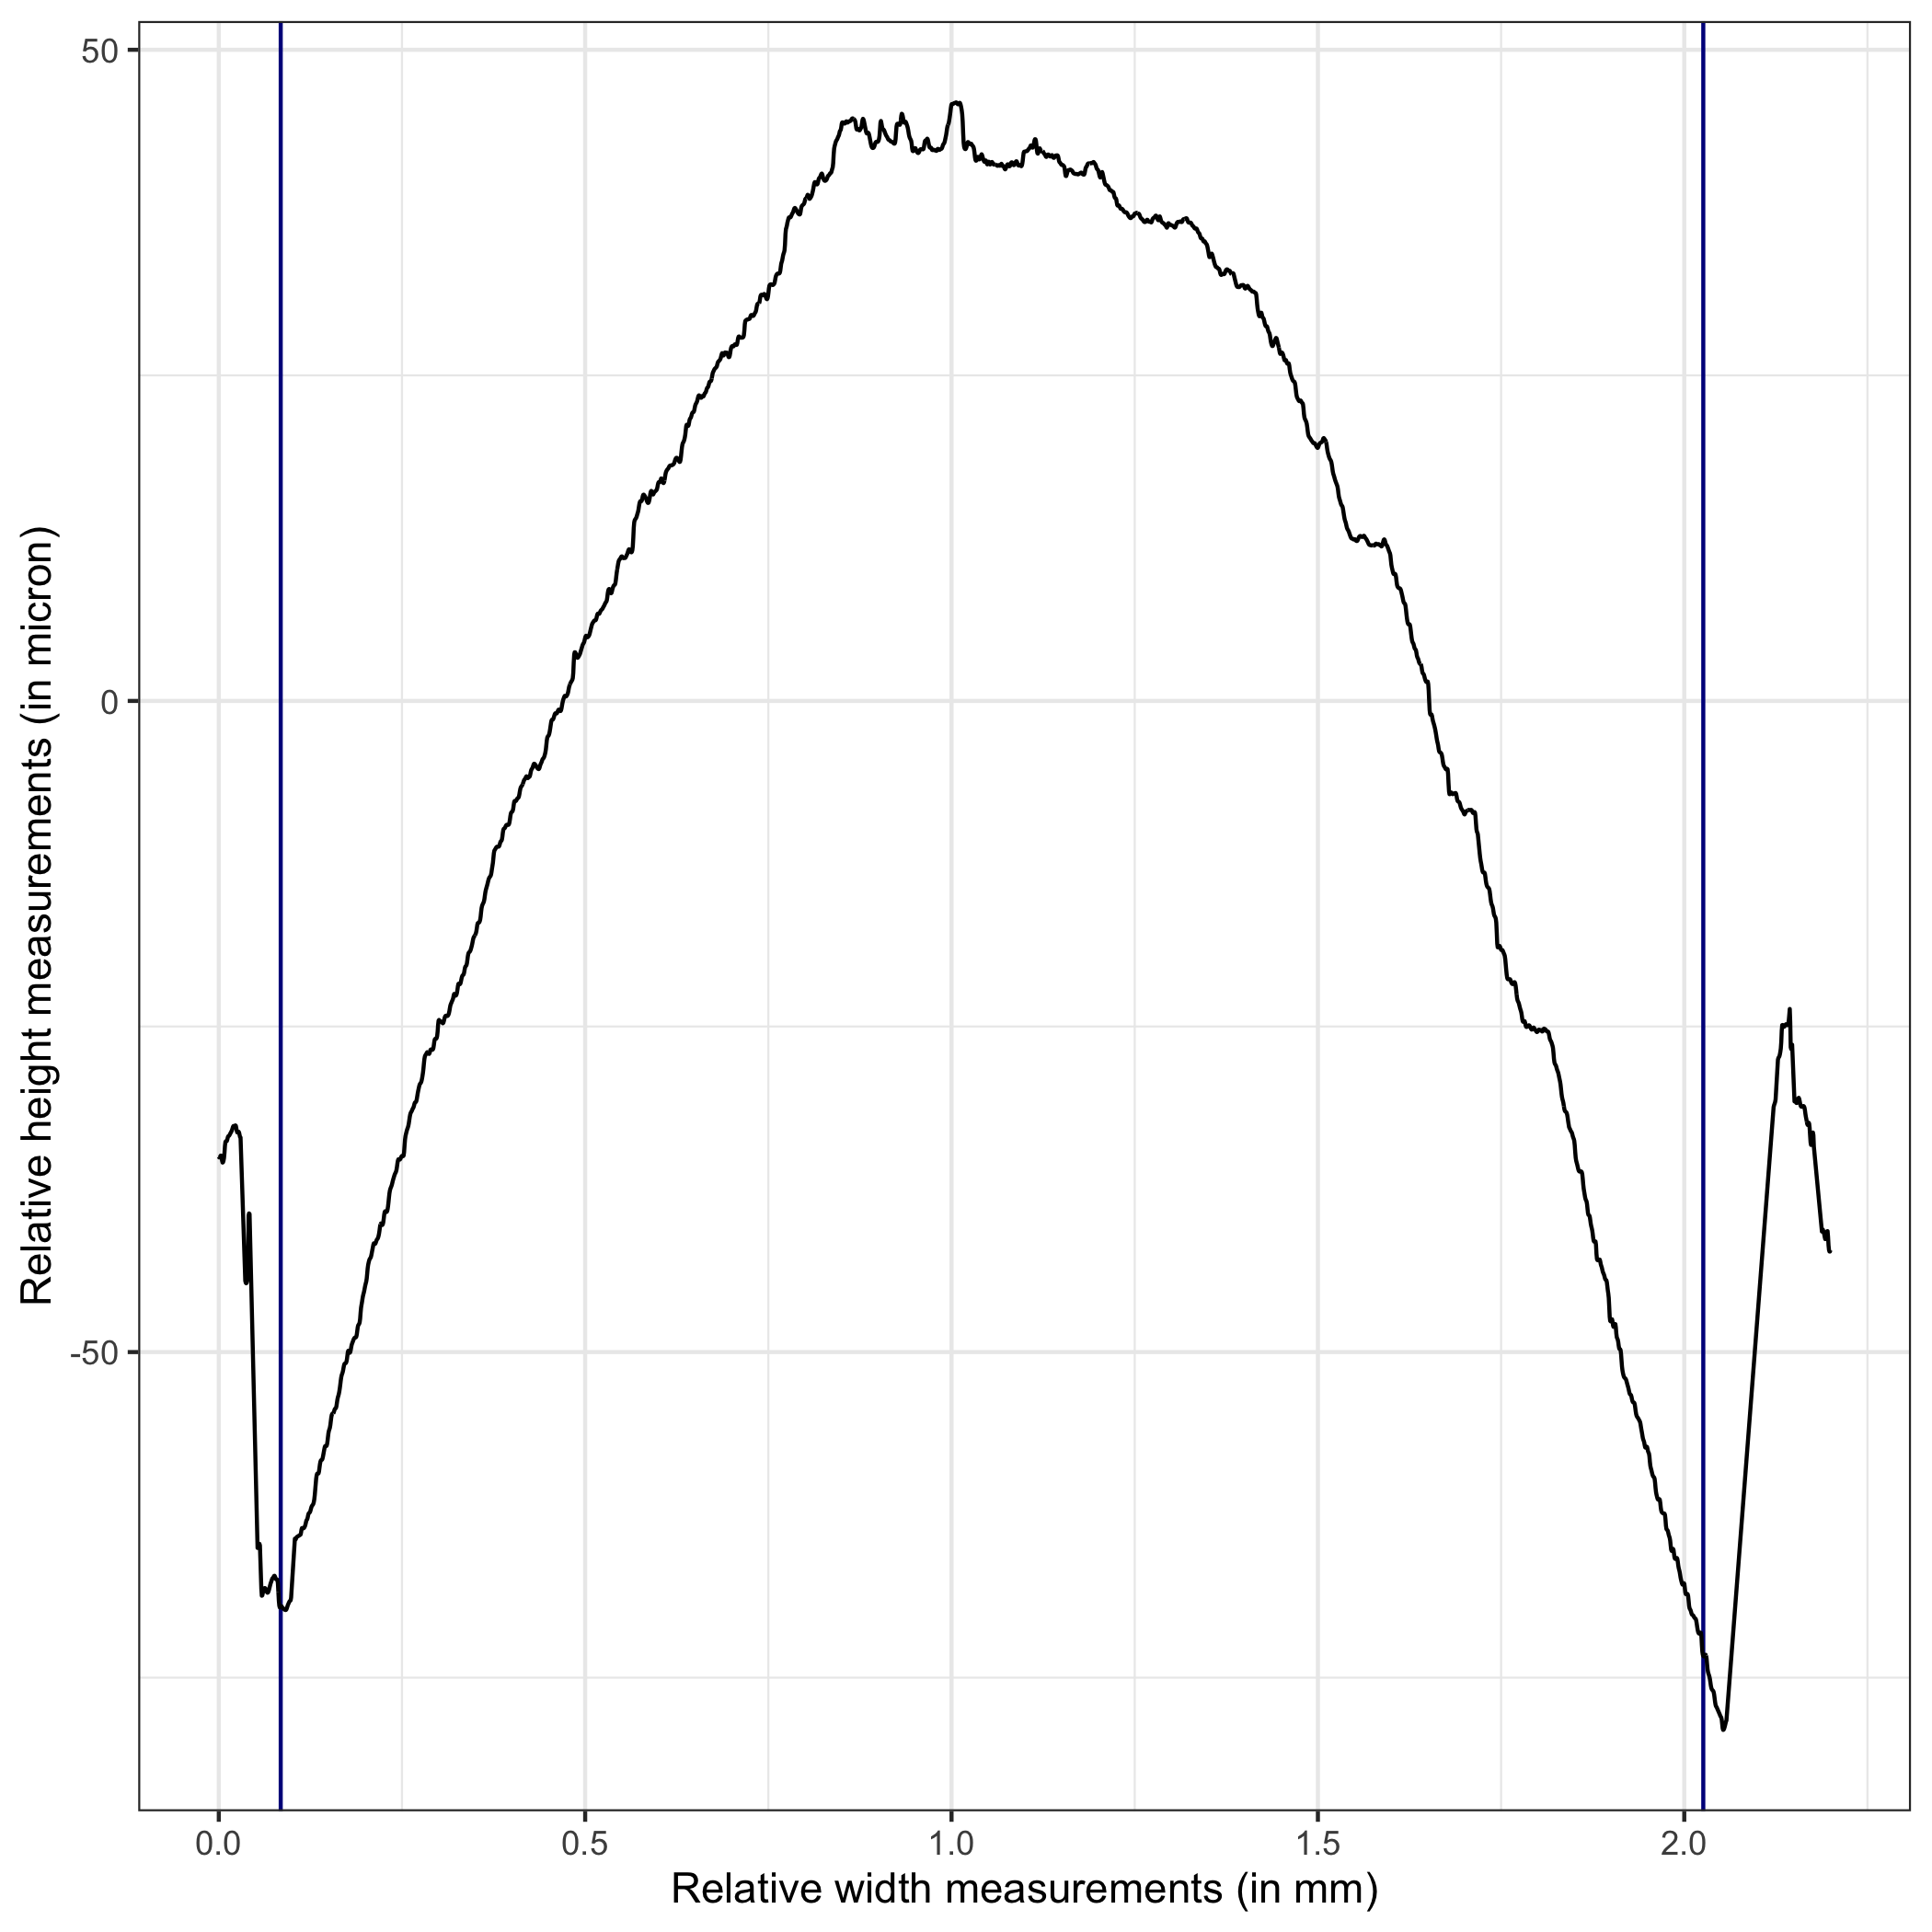
\includegraphics[width=\maxwidth]{figure/crosscut-motivation-1} 

}

\caption[Profile of a land engraved area (LEA), left and right groove locations are marked as vertical lines]{Profile of a land engraved area (LEA), left and right groove locations are marked as vertical lines.}\label{fig:crosscut-motivation}
\end{figure}


\end{knitrout}


The predominant feature of this crosscut is the curvature of the barrel as well as two deep trenches next to two peaks which represent the beginning of the shoulders of the bullet land. To extract a signature from this data, the curvature of the bullet structure must be removed, leaving behind clear indications of striae. To accomplish this task, \cite{hare2017} fit a loess regression to the data. The residuals of this regression are then considered to be the signature of the particular bullet land in question. Due to the high variability in height of the bullet grooves or shoulder area of the bullet land, inclusion of these regions would significantly decrease the quality of the loess regression estimate of the bullet curvature since these regions are highly influential. 

\begin{knitrout}
\definecolor{shadecolor}{rgb}{0.969, 0.969, 0.969}\color{fgcolor}\begin{figure}[H]

{\centering \includegraphics[width=\maxwidth]{figure/signal-motivation-1} 

}

\caption[Signatures corresponding to the above profile with properly specified and improperly specified locations of the left groove]{Signatures corresponding to the above profile with properly specified and improperly specified locations of the left groove.}\label{fig:signal-motivation}
\end{figure}


\end{knitrout}

% 
% <<signal-motivation-good, echo = FALSE, fig.align="center", message=FALSE, warning = F, fig.height = 3, fig.cap= "Single signature with properly identified groove engraved areas">>=
% 
% sigs1 <- cc_get_signature(ccdata, grooves, span1 = 0.75, span2 = 0.3)
% 
% sigs1 %>% 
%   dplyr::filter(!is.na(sig),!is.na(raw_sig)) %>%
%   ggplot(aes(x = x)) + 
%   geom_line(aes(y = raw_sig), colour = "grey30") +
%   geom_line(aes(y = sig), colour = "grey70") +
%   ylim(c(-5,5)) +
%   theme_bw()
% 
% @
% 
% 
% <<signal-motivation-bad, echo = FALSE, fig.align="center", message=FALSE, warning = F, fig.height = 3, fig.cap= "Single signature with improperly identified groove engraved areas">>=
% grooves.bad <- list("groove" = c(grooves$groove[1] -50, grooves$groove[2] - 50))
% 
% sigs2 <- cc_get_signature(ccdata, grooves.bad, span1 = 0.75, span2 = 0.3)
% 
% sigs2 %>% 
%   dplyr::filter(!is.na(sig),!is.na(raw_sig)) %>%
%   ggplot(aes(x = x)) + 
%   geom_line(aes(y = raw_sig), colour = "grey30") +
%   geom_line(aes(y = sig), colour = "grey70") +
%   ylim(c(-5,5)) +
%   theme_bw()
% 
% @
% 

% \begin{figure}[ht!]
% \begin{subfigure}{.5\textwidth}
%   \centering
%   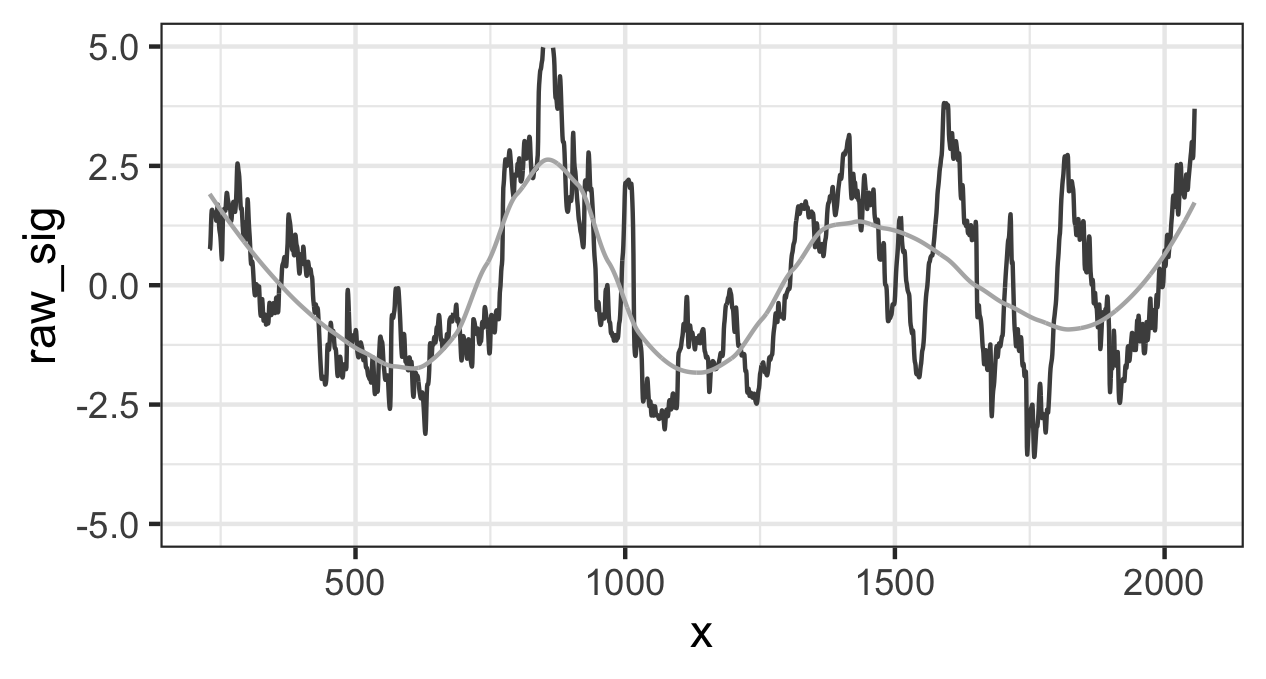
\includegraphics{../images/signal-motivating-example-good-grooves.png}
%   \caption{A signature extracted from the Hamby 44 set barrel 7, bullet 1, land 3 with properly removed grooves}
% \end{subfigure}
% \begin{subfigure}{.5\textwidth}
%   \centering
%   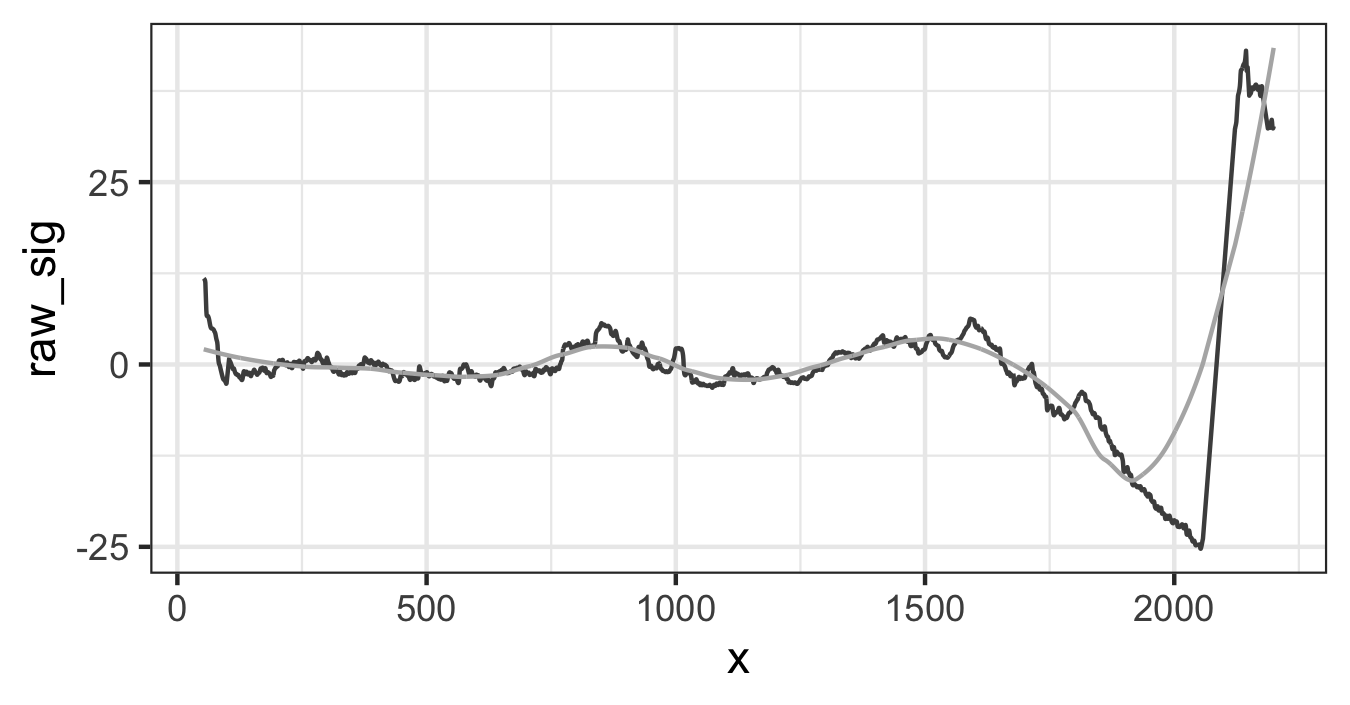
\includegraphics{../images/signal-motivating-example-bad-grooves.png}
%   \caption{A signature extracted from the Hamby 44 set barrel 7, bullet 1, land 3 with improperly removed grooves}
% \end{subfigure}
%     \label{fig:sig-comparison}
% \end{figure}

In Figures \ref{fig:signal-motivation-good} and \ref{fig:signal-motivation-bad} we see a comparison between two signatures one where the grooves are properly identified and one where the grooves are improperly identified. When the right-hand groove is included the residuals are dominated by the bullet groove and the striae are no longer as pronounced. So accurately identifying the bullet grooves is supremely important for bullet identification. We propose a new method for identifying bullet grooves that utilizes an image analysis technique known as the Hough transform to identify prominent features of the bullet land. 


\subsection{Data}

Data for this project comes from two primary sources, Hamby Set 44 and Phoenix PD set provided by Tylor Klep.  As explained in \cite{Vanderplas2020}, the Hamby Set 44 consists of a total of 35 bullets fired through ten consecutively manufactured Rugers P85s. This set consists of 20 known bullets and fifteen bullets of unknown origin from the ten barrels in this set. Ammunition for this set was 9 mm Lger 115 Grain Full Metal Jacket from the Winchester Ammunition Company. The Phoenix PD set consists of three test fires from each of eight different consecutively rifled Ruger P-95 barrels. In addition, there are ten questioned bullets provided and it is not known whether any of the questioned bullets are fired from the known barrels. Bullets for this set are American Eagle 9 mm Luger full metal jackets and were scanned by Bill Henderson of Sensofar.


\subsection{Background}

While not specifically targeted at identifying bullet land grooves, image processing techniques have been applied in previous work to enhance and identify usable striae.  \citet{chu2010} create a metric for identifying the quality of 3-dimensional bullet scans using two metrics they called ``striation density" and ``edge density". Researchers define ``edge density" to be the ratio between the number of pixels detected on an edge and the total number of pixels in the area. Next they utilize some form of threshold filter to identify which edges are striae, and define ``striation density" as the ratio between the number of pixels on the identified striations and the total number of pixels in the area. They argue that scans with a higher ``striation density" will be better candidates for examination and identification. 

In a later work  by \citet{chu2013} image processing techniques were taken a step further. Rather than using edge detection to establish a quality metric, edge detection was used to identify the location of valid striation marks. Once the location of striae were known, a mask that covered and expanded the edge points of valid striae was utilized to identify areas of bullet scans that would be suitable for use in a CCF (cross correlation function) analysis. CCF has previously been studied \cite{chu2010-ccf} and found to be a useful method for bullet identification. So the ability to identify where CCF can be applied is a step forward on the path to automated identification of bullet lands. However, these methods identified in \cite{chu2013} are not available in algorithmic form to researchers outside of the National Institute of Standards and Technology(NIST), making it difficult to verify results.  

While not explicitly stated in this work, the images in \cite{chu2013} make it clear that all of the bullet images upon which the researchers are running their edge detection methods have the Groove Engraved Areas (GEAs) of the bullet scan removed. While no method for groove identification is proposed in the three previous research publications cited, it is reasonable to speculate that such areas were manually identified. If so, this highlights the need for automated and unbiased identification of groove engraved areas since the identification of the LEA in bullet scans on the scale necessary to create some sort of database is time intensive and also introduces another element of human intervention in the bullet identification process. Part of the problem with the existing research presented in this paper is that the methods are not described in enough detail to allow for replication of results from external researchers. In addition, the manual intervention results implicit in \cit{chu2013} are not available for public scrutiny or use. 


To evaluate the accuracy of our groove identification we will use a metric devised by Kiegan Rice, Nate Garton, and Heike Hofmann (citation needed). The idea behind this metric is that a robust LOESS is fit to model the curvature of the bullet scan using the following process. A residual is then calculated between the predicted robust LOESS fit of the bullet curvature and the actual data. Then the area between the predicted groove location and the manually identified groove location is examined and the sum of the absolute values of the robust LOESS residual multiplied by the resolution of the scan yields an area in microns. This area is the area of mis-identification and can be used as a score to judge how closely our estimated groove location is to the manually identified groove location. 
\hh{ Discussion on resulting units and formula for loess needed}

\subsection{Brief Overview of Hough Transforms}


In broad terms, the Hough Transform is a feature extraction technique for detecting shapes in an image. For any given point in the (x,y)-plane of our image we can calculate a corresponding line in the feature space as shown in Figure~\ref{fig:parameterization}. Points that lie on the same line will have lines that intersect in the feature space. 
\begin{figure}[!ht]
\begin{subfigure}{.5\textwidth}
\centering
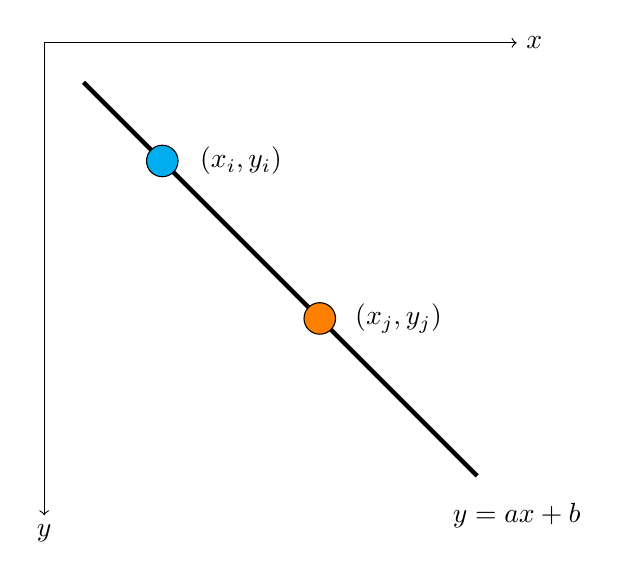
\begin{tikzpicture}
\draw [<->] (0,-6) node (yaxis) [below] {$y$} -- (0,0) -- (6,0) node (xaxis) [right] {$x$};
\draw [ultra thick] (0.5,-0.5) -- (5.5, -5.5);
\draw [fill = cyan] (1.5,-1.5) circle [radius=0.2];
\node [] at (2.5, -1.5) {($x_{i}, y_{i}$)};
\draw [fill = orange] (3.5,-3.5) circle [radius=0.2];
\node [] at (4.5, -3.5) {($x_{j}, y_{j}$)};
\node [] at (6,-6) {$y = ax + b$};
\end{tikzpicture}
\label{fig:tikz1}
\end{subfigure}
\begin{subfigure}{.5\textwidth}
\centering
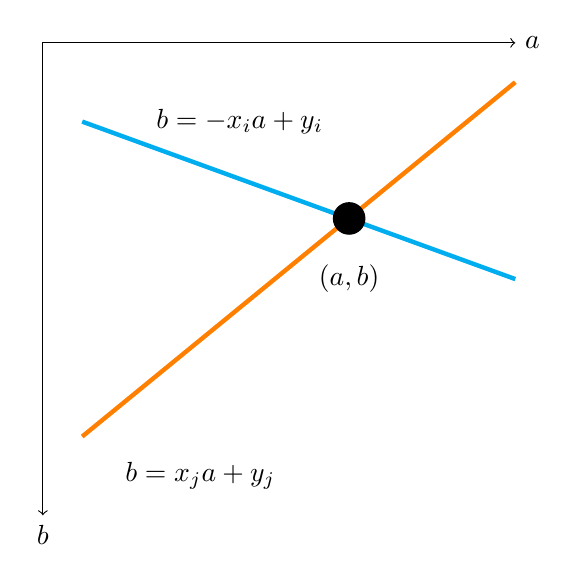
\begin{tikzpicture}
\draw [<->] (0,-6) node (yaxis) [below] {$b$} -- (0,0) -- (6,0) node (xaxis) [right] {$a$};
\draw[cyan, ultra thick] (0.5, -1) -- (6,-3);
\node [] at (2, -5.5) {$b=x_{j}a + y_{j}$};
\node [] at (2.5, -1) {$b=-x_{i}a + y_{i}$};
\draw[orange, ultra thick] (0.5, -5) -- (6,-0.5);
\draw [fill] (3.89,-2.23) circle [radius=0.2];
\node [] at (3.89, -3) {($a, b$)};
\end{tikzpicture}
\label{fig:tikz2}
\end{subfigure}
\caption{Diagram of feature space linea transformation oriented for image origin.}
\label{fig:parametrization}
\end{figure}


The point of intersection in the feature space, then corresponds to the parameters used to describe the edge in the (x,y)-plane that the two detected points lie upon. A two dimensional array called the ``accumulator array" is used to keep track of features detected.  The accumulator array covers the entirety of the feature space separated into a user-specified number of bins. For each set of features detected the bin in the accumulator array associated with that set of features is incremented. So in theory, strong features should have higher values in their associated bin because there is a larger number of pixels detected that all have the same set of features in the feature space. 

 When we are performing our Hough algorithm, we do not use the actual x3p-file we transform the data into a two-dimensional image. In the two-dimensional representations of bullet images, the y-axis is inverted from the standard x-y plane. A reason for this is that the images are processed in \textbf{C++} which stores images, known as ``CImgs''(Cool Images) in a vector format where the first pixel in the vector corresponds to the upper left-hand pixel of the image located at (0,0). Pixels are then ordered from left to right, extending from the origin to the positive x-direction and from top to bottom, from the x-axis towards the negative y-direction.
 
\section{Methods}


In order to best identify the GEAs we first want to diminish noise in the image. This can be achieved by converting each scan into an image gradient, which signifies where there are directional changes in the color of the image. This approach unfortunately loses most of the detail of the three dimensional scans, however, it better highlights the differences between LEAs and GEAs. Once an image gradient is obtained we select only edges we consider to be ``strong", meaning they have a magnitude above the 99th percentile. Our reason for not fully carrying out a Canny Edge detection algorithm before using a Hough transform is that the Canny Edge algorithm increases processing time by about 35 seconds per image and actually highlights more striae and break-off. 

\begin{knitrout}
\definecolor{shadecolor}{rgb}{0.969, 0.969, 0.969}\color{fgcolor}\begin{figure}[H]

{\centering \includegraphics[width=\maxwidth]{figure/strong-edge-1} 

}

\caption[Land Engraved Areas with Edges with magnitudes in the 99th percentile]{Land Engraved Areas with Edges with magnitudes in the 99th percentile}\label{fig:strong-edge}
\end{figure}


\end{knitrout}

\begin{knitrout}
\definecolor{shadecolor}{rgb}{0.969, 0.969, 0.969}\color{fgcolor}\begin{figure}[H]

{\centering \includegraphics[width=\maxwidth]{figure/canny-edge-1} 

}

\caption[Land Engraved Areas with Edges enhanced with Canny Edge Detection]{Land Engraved Areas with Edges enhanced with Canny Edge Detection}\label{fig:canny-edge}
\end{figure}


\end{knitrout}

As shown in Figure \ref{fig:canny-edge} the striae in the LEA are much more pronounced than in the image with only strong edges. We wish to focus on only detecting GEAs, so detecting an increased number of striae through Canny edge detection is not useful for our algorithm. Once we obtain the image gradient with only the strong edges we can then utilize our Hough transformation to obtain generally reasonable estimates of image boundaries. For the Hough transformation we utilize the function `` \texttt{hough\char`_lines}" from the imager package with the number of bins set to 100. While changing the number of bins does not seem to effect the processing time of the Hough transform, having a larger number of bins increases the number of extraneous detected lines in the image. 

We make the assumption that scans are oriented properly and as such, most Hough lines that correlate to the GEAs will be roughly vertical with some deviations in angle based on scanning technique. It is worth noting that the original output of the `` \texttt{hough\char`_lines}" functions have angles ranging from 0 to $2\pi$. So to make selecting lines from our desired range, easier we chose to transform any angle greater than $\pi$, to instead be from 0 to $-\pi$ by subtracting $2\pi$ from the original theta angle. Therefore we select only the Hough lines that have theta angles from the positive x-axis less than $\frac{\pi}{16}$ and greater than $\frac{-\pi}{16}$. The parametrization produced by `` \texttt{hough\char`_lines}" is of the form:

\begin{center}
$\rho = x \ cos(\theta) \ + \ y \ sin(\theta)$
\end{center}

Where $\rho$ represents the length of the normalized orthogonal vector between the detected line and the origin of the image, and $\theta$ is the angle between the positive x-axis and the normalized vector. In Figure \ref{fig:hessian-graphic-inclusion} we see an example of how Hough transforms parametrize a line. The orange line represents an example of a detected Hough line. The teal line connecting the origin to the orthogonal bisector of our detected Hough line represents the vector denoted $\rho$ in our above equation. Similarly the teal arc below represents the angle, $\theta$, which is the difference between the top of the image and the orthogonal bisector. 



\begin{knitrout}
\definecolor{shadecolor}{rgb}{0.969, 0.969, 0.969}\color{fgcolor}\begin{figure}[H]

{\centering 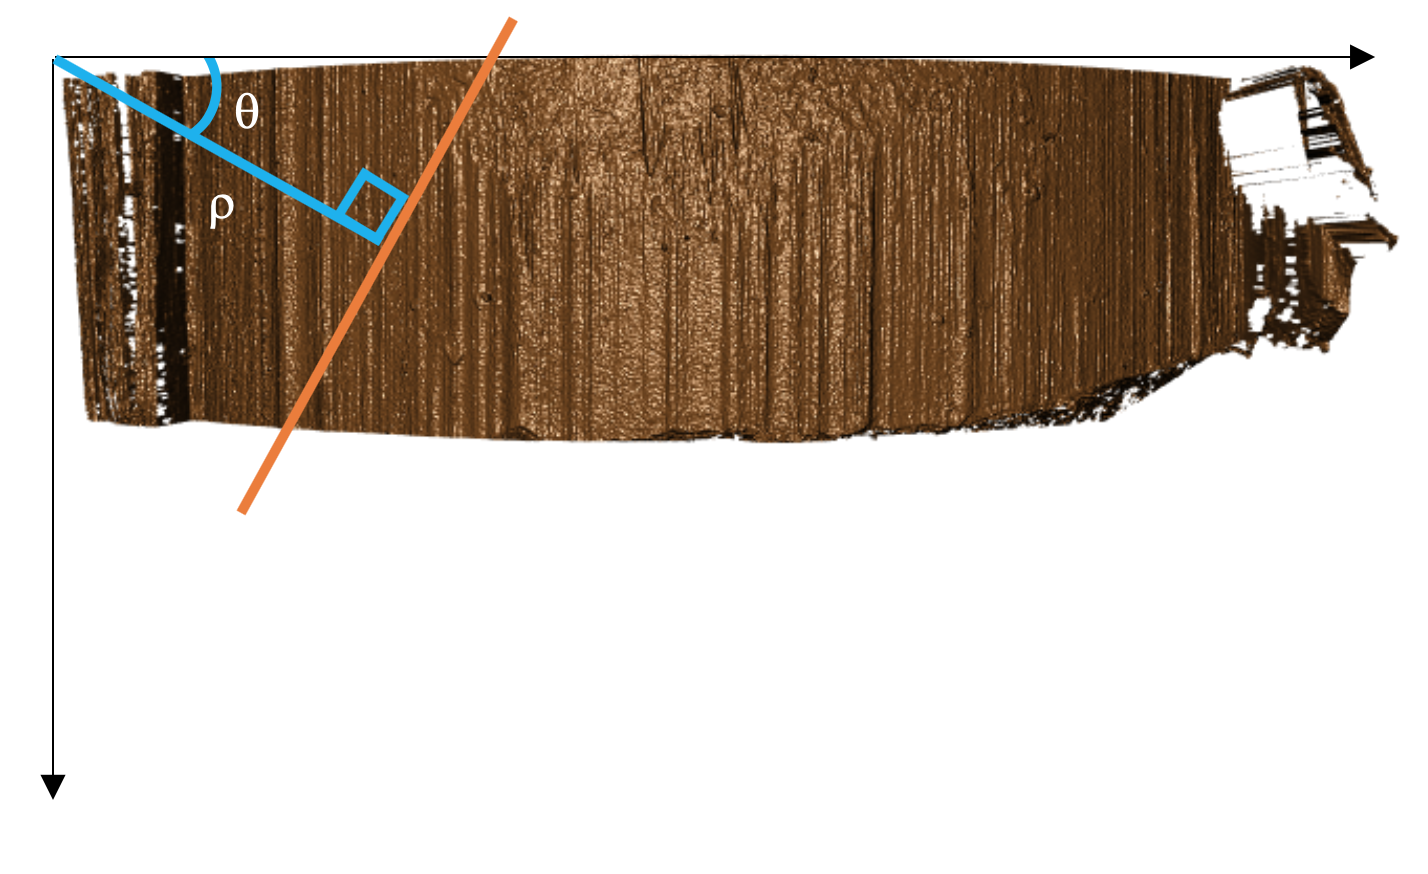
\includegraphics[width=0.8\linewidth]{../images/hessian-example} 

}

\caption[Example of Hessian Normal Form parametrization overlaid a bullet scan]{Example of Hessian Normal Form parametrization overlaid a bullet scan}\label{fig:hessian-graphic-inclusion}
\end{figure}


\end{knitrout}

We take a moment here to define a couple of symbols for use in our explanation to follow:
\begin{itemize}
  \item $\mathbf{x_{t}}$: The x-intercept at the top of the bullet land \\
  \item $\mathbf{x_{b}}$: The x-intercept at the bottom of the bullet land \\
  \item $\boldsymbol\delta$: The difference between $x_t$ and $x_b$ in the x-direction \\
  \item \textbf{h}: The height of the bullet land \\
  \item $\mathbf{m_y}$: The slope of the detected Hough line in the y-direction \\
  \item $\mathbf{m_x}$: The slope of the detected Hough line in the x-direction \\
\end{itemize}
We note that when $\theta$ is equal to 0, the $x_t$ is given by $\rho$ however when $\theta$ is not 0 we utilize the above equation to find that the 
\begin{center}
$x_t$ = $\frac{\rho}{\cos(\theta)}$
\end{center}

We utilize this calculation to find where the estimated Hough line intersects the top and bottom of the bullet land. The $x_t$ was calculated previously, however to calculate $x_b$ we utilize some geometric properties. We can draw a perpendicular line from the $x_t$ to $x_b$ creating a right triangle as shown below in Figure \ref{fig:xbottom-graphic-inclusion}. Since both the angle between the orthogonal bisector labeled $\rho$ and the new triangle created from the $x_t$ to the bottom of the land are both right triangles, we know that the angle at the top of the newly formed triangle is equivalent to $\theta$. Since the $x_t$ is known, we can use an elementary geometry technique to calculate the distance labeled $\delta$ in the diagram below. Since $\tan(\theta)$ is equivalent to the proportion of the length of the ``opposite" side over the ``adjacent" side of the right triangle, we know that $\delta = \tan(\theta)*\text{h}$. So then $x_b = x_t - \delta$. 



\begin{knitrout}
\definecolor{shadecolor}{rgb}{0.969, 0.969, 0.969}\color{fgcolor}\begin{figure}[H]

{\centering 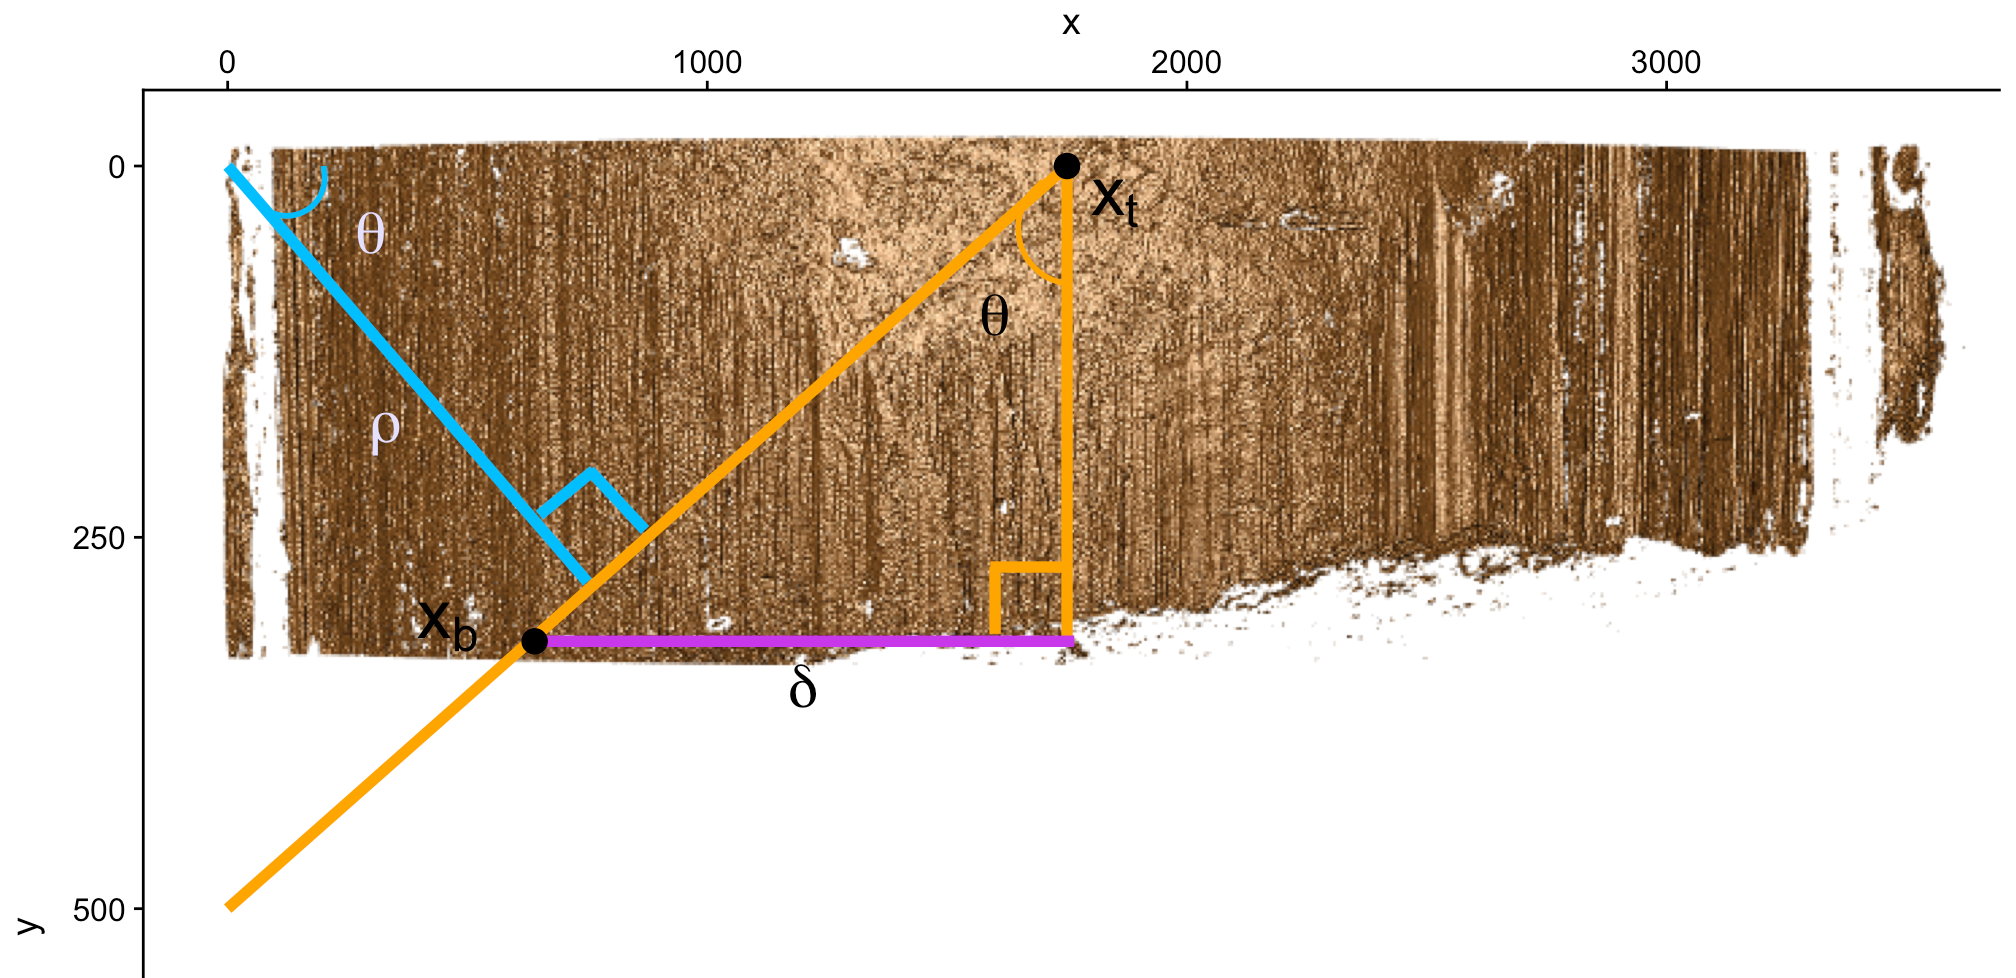
\includegraphics[width=0.8\linewidth]{../images/calc-xbottom} 

}

\caption[Demonstration of calculation of bottom intercept of a bullet land using SOH-CAH-TOA]{Demonstration of calculation of bottom intercept of a bullet land using SOH-CAH-TOA}\label{fig:xbottom-graphic-inclusion}
\end{figure}


\end{knitrout}

The utility for calculating the top and bottom intercept of our bullet land is that it allows us to calculate the slope of each Hough line with respect to the y-direction. 
\begin{center}
 $m_y = \frac{(x_t - x_b)}{\text{h}}$
\end{center}

Traditionally $m_x$ is chosen for describing the equation of a line, however, because we are primarily interested in vertical lines $m_x$ tends to infinity. This is undesirable because our end goal is to be able to identify the location of a bullet groove at a particular location on the y-axis, a crosscut. To identify the x-location of the groove for a given crosscut of our bullet scans, we want to input the y-location of the crosscut to our linear equation estimate of the groove and solve for x. So a slope of infinity makes this process hard to automate when we can eliminate this problem by simply having a slope in the y-direction. 

As discussed before, the Hough transform outputs a score that corresponds to the number of pixels detected on a line that can give us an indication of the strength of the feature detected. Theoretically, we would expect the strongest lines in our image to be the grooves on either side of the bullet land. So the problem arises of how best to select strong edges. Rather than simply filter scores on some arbitrary threshold, we normalize the Hough scores by the largest possible score that could be achieved for each set of features detected. The reason for this is that longer lines will have a larger Hough score simply by virtue of having a larger number of possible detectable pixels. So if we want to compare the strength of various lines, regardless of line length, we need to normalize each score associated with each line detected.  



\begin{knitrout}
\definecolor{shadecolor}{rgb}{0.969, 0.969, 0.969}\color{fgcolor}\begin{figure}[H]

{\centering 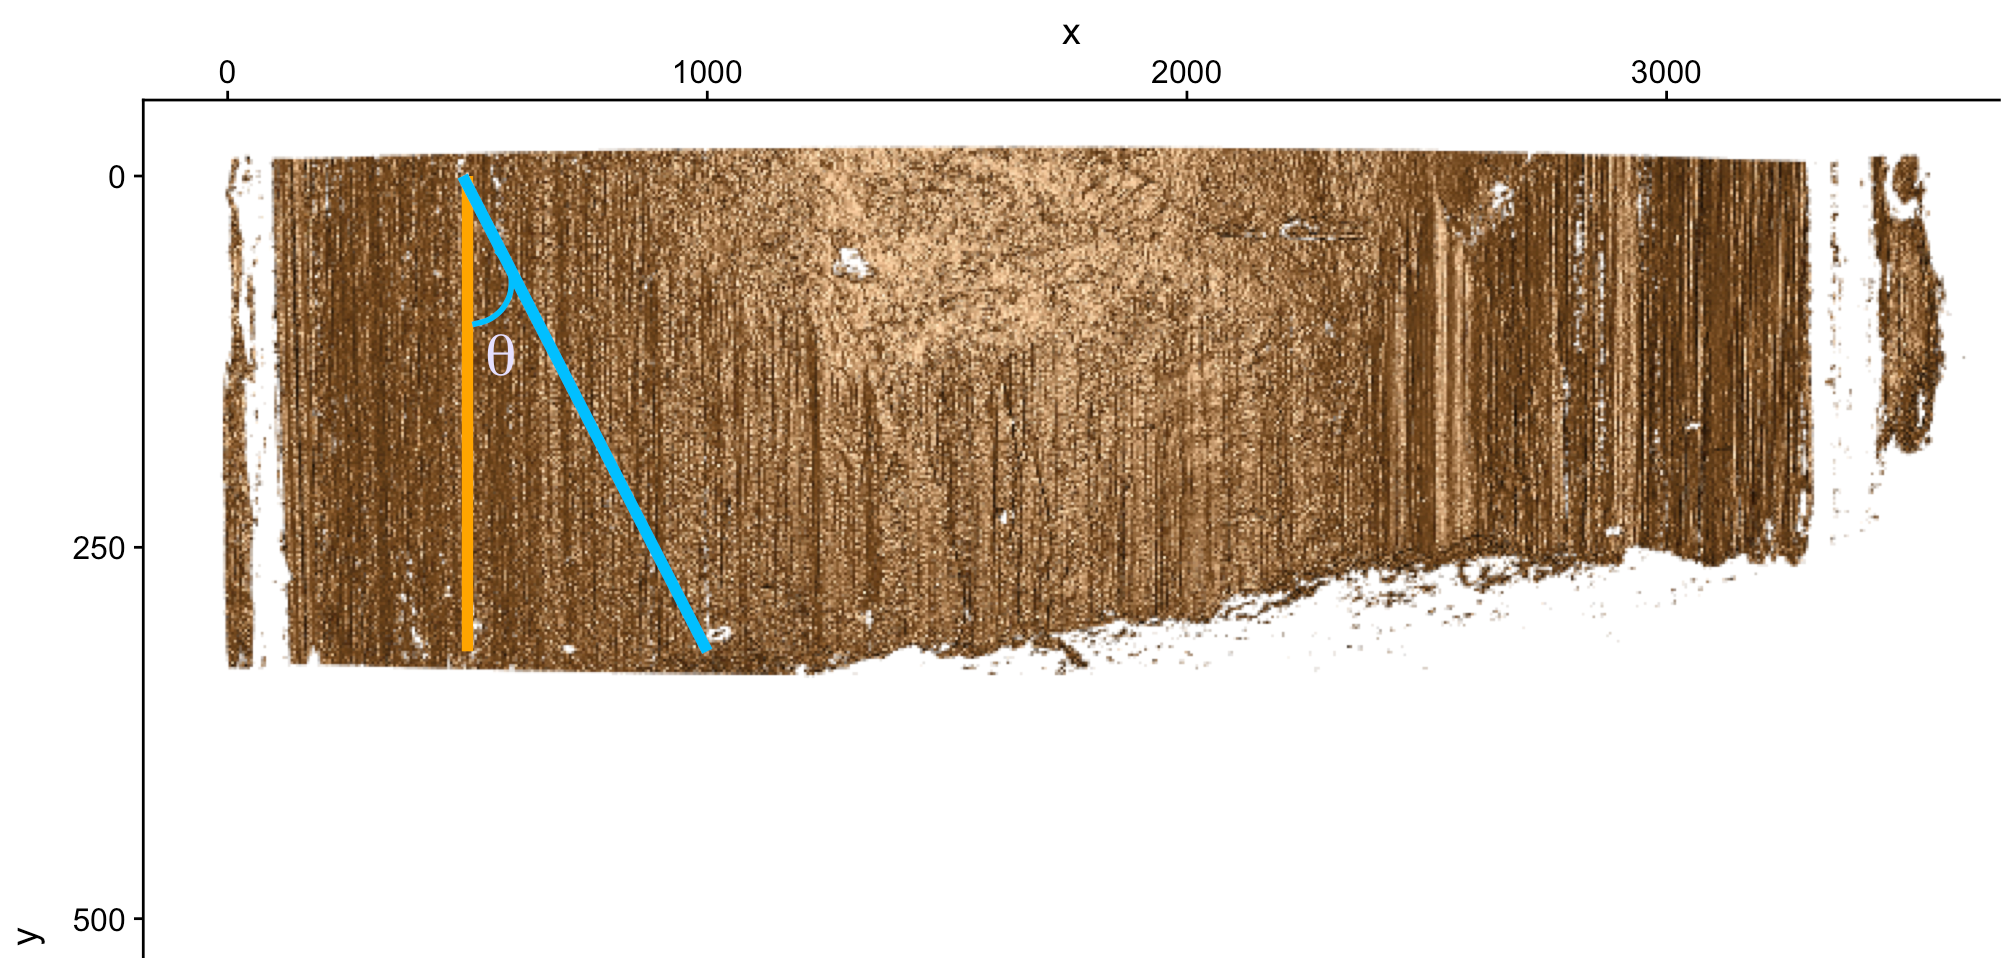
\includegraphics[width=0.8\linewidth]{../images/calc-theoretical-max} 

}

\caption[Demonstration of calculation of theoretical maximum score]{Demonstration of calculation of theoretical maximum score}\label{fig:max-graphic-inclusion}
\end{figure}


\end{knitrout}


We calculate the largest possible theoretical score($\psi_{max}$) using the following.
\begin{center}
  $\psi_{max} = \frac{h}{\cos(\theta)}$
\end{center}
This should in theory give us the total possible pixels that the Hough transform could have detected in our image by exploiting geometric properties of the right triangle shown in Figure~\ref{fig:max-graphic-inclusion}. Then for each unique set of features that describe a line that the Hough transform detects we divide the score associated with these features($\psi$) by the theoretical maximum score, yielding the normalized score($\psi_{norm}$).
\begin{center}
 $\psi_{norm} = \frac{\psi}{\psi_{max}}$
\end{center}

\begin{knitrout}
\definecolor{shadecolor}{rgb}{0.969, 0.969, 0.969}\color{fgcolor}\begin{figure}[H]

{\centering \includegraphics[width=\maxwidth]{figure/middle-fifty-1} 

}

\caption[Land Engraved Areas with Edges with magnitudes in the 99th percentile]{Land Engraved Areas with Edges with magnitudes in the 99th percentile}\label{fig:middle-fifty}
\end{figure}


\end{knitrout}

% \begin{figure}[ht!]
%   \centering
%   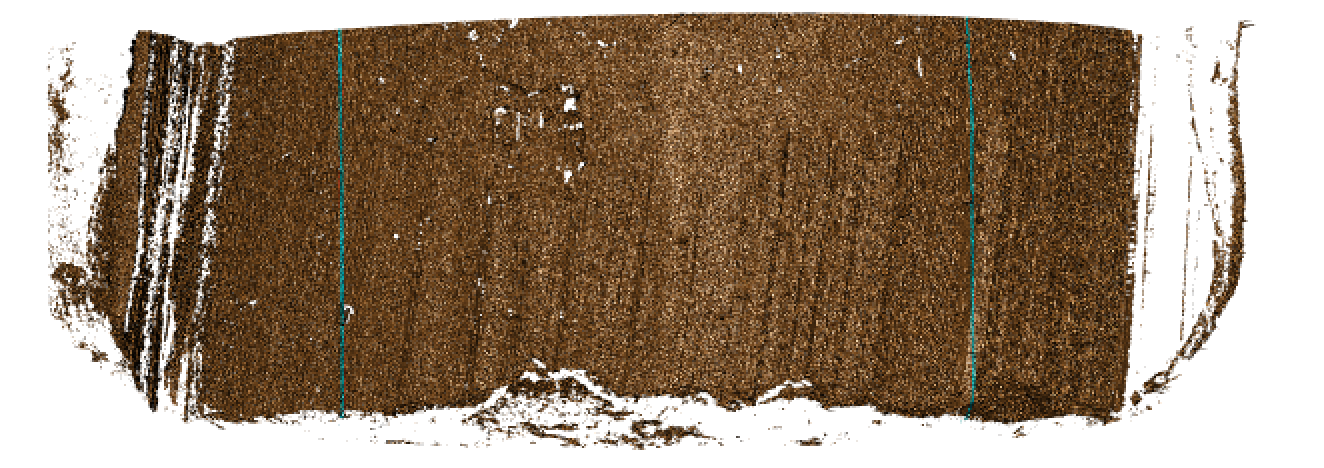
\includegraphics{../images/phnx-1-m2-b1-l1-middle-fifty-demo.png}
%   \caption{Middle fifty percent of the bullet land marked by two cyan coloured vertical lines imposed over the Phoenix set Gun 1-M2 Bullet 1 Land 1 scan}
%   \label{fig:middlefifty}
% \end{figure}

To further specify the best candidates for the bullet land grooves, we rely on the heuristic that most of the middle 50\% of the bullet will be occupied by striae. Therefore, we can eliminate any strong lines detected within this region. An example of the middle fifty percent of a bullet land can be seen in Figure \ref{fig:middle-fifty} where the middle fifty percent of the bullet land is bordered by green colored vertical lines. We note that the grooves are well away from this middle fifty percent region, making this a suitable heuristic. We then select the highest normalized score of the lines detected outside of the middle fifty percent of the bullet land. We claim then that this is our detected bullet groove. If on the off chance that the strongest feature detected is within the middle 50\% area of the bullet land, then the grooves are set to be the borders of the middle 50\% area. 

Once features are chosen to describe both the left and right hand grooves of the bullet land the `get\_grooves\_hough` function translates these features into two equations for lines. It is worthwhile to note at this point that our calculations have been in terms of pixels detected in an image rather than the microns of the bullet scan. So we must transform our equations of lines from being in terms of pixels to microns. This is accomplished inside the `get\_grooves\_hough` function by the helper function `pix\_to\_micron` which subtracts one from the pixel location (since pixels start indexed at one and microns start indexed at zero), then multiplies that pixel location by the resolution of the x3p-scan($r_s$). Because we are interested in the slope with respect to the y-direction we calculate our linear equations as follows, where $y_i$ is any y-location on the bullet land:

\begin{center}
  $\text{Groove Estimate} = (x_b -1)*r_s + m_y*y_{i} - \text{adjust}$
\end{center}

 Unlike other methods available in the `GrooveFinder` package, the `get\_grooves\_hough` function does not provide a groove estimate at an optimized crosscut. The output of the  `get\_grooves\_hough` function are a set of two functions that correspond to the left and right-hand grooves. So to produce an actual estimate of our groove location we need to input a y-location into our two functions. For a single point-estimate we can input the y-location of a single crosscut using the `x3p\_optimize\_crosscut` function from the `bulletxtrctr` package. However to visualize our groove estimates across the entire bullet land we have created a helper function called `get\_mask\_hough` that creates a colored mask over our bullet land of our groove estimates as shown in Figure \ref{fig:get-mask-hough-example}. 
 


\begin{knitrout}
\definecolor{shadecolor}{rgb}{0.969, 0.969, 0.969}\color{fgcolor}\begin{figure}[H]

{\centering 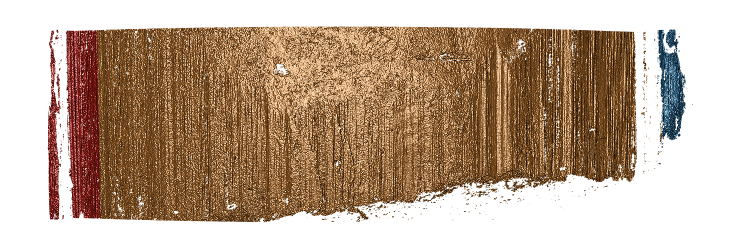
\includegraphics[width=\maxwidth]{../images/mask-example} 

}

\caption[Hough groove estimate visualized over whole of bullet land with adjust set to 120]{Hough groove estimate visualized over whole of bullet land with adjust set to 120}\label{fig:get-mask-hough-example}
\end{figure}


\end{knitrout}
 


\section{Results}

In order to assess the effectiveness of the Hough Transform method we will use the ``Area of Misidentifiaction" score, as described above, to see how far away our prediction is from the manually identified groove location. We will also compare our results to one other method of groove identification to see how well this new method compares to tools previously developed by CSAFE researchers. In total there will be two methods for comparison:

\begin{enumerate}
\item Hough Transform
\item Rollapply
\end{enumerate}

Scores were obtained for two different bullet test sets, the Phoenix PD set, and the Hamby 44 set. Due to the sheer size of the individual x3p files in each set, scores were obtained for each file one at a time. An x3p file would be read into local memory and three different groove locations would be calculated for each method identified above. Then a robust LOESS is fit to the x3p file to remove bullet curvature and signatures are extracted. The area of misidentification in microns is calculated for each of the three methods for each groove (left and right) and stored in the form of a dataset. This process is repeated for every file in the test set, where scores are stored and appended into a large dataframe of scores, groove locations, manual identification locations, and bullet identifications. Ideally, well identified grooves should have an area of misidentification close to zero for both the left and right grooves. 

To improve the accuracy of the Hough transform, we have decide to impute areas of missing information in bullet lands. Missing information in the land is filled in with a value that is 5\% greater than the maximum height value detected in the bullet land.



\begin{knitrout}
\definecolor{shadecolor}{rgb}{0.969, 0.969, 0.969}\color{fgcolor}\begin{figure}[H]

{\centering 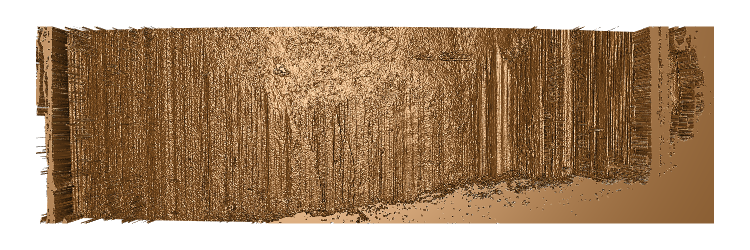
\includegraphics[width=\maxwidth]{../images/fill-na-example} 

}

\caption[Bullet Land with missing values imputed]{Bullet Land with missing values imputed}\label{fig:five-percent-imputed}
\end{figure}


\end{knitrout}
 
 
Below we present the distribution of area of misidentification(AOM) scores for Hough and Rollapply estimates for the Phoenix PD set. In the below figure Hough estimate scores for area of misidentification are shown in orange and scores for Rollapply are shown in blue. Smaller logged scores indicate a more accurate identification of groove locations. For both the right and left-hand grooves for this set we see that the Hough method has a smaller spread in logged AOM scores than the rollapply method. For the left hand groove, the Hough method appears to have a lower median logged AOM score than the rollapply method however for the right hand side, the median logged AOM scores is slightly higher. 

\begin{knitrout}
\definecolor{shadecolor}{rgb}{0.969, 0.969, 0.969}\color{fgcolor}\begin{figure}[H]

{\centering \includegraphics[width=\maxwidth]{figure/phoenix-lh-score-dist-1} 

}

\caption[Boxplots of AOM scores for the Phoenix PD set separated by groove side and method]{Boxplots of AOM scores for the Phoenix PD set separated by groove side and method}\label{fig:phoenix-lh-score-dist}
\end{figure}


\end{knitrout}



We see similar results in the Hamby 44 Set for both the left-hand and right-hand groove estimates. In figure [insert figure number ere] 

\begin{knitrout}
\definecolor{shadecolor}{rgb}{0.969, 0.969, 0.969}\color{fgcolor}\begin{figure}[H]

{\centering \includegraphics[width=\maxwidth]{figure/hamby44-lh-score-dist-1} 

}

\caption[Distribution of left-hand areas of misidentification for Hamby 44 Set]{Distribution of left-hand areas of misidentification for Hamby 44 Set}\label{fig:hamby44-lh-score-dist}
\end{figure}


\end{knitrout}

\bibliography{summat} % Tells it where your list of references is.
\bibliographystyle{plainnat} 

\end{document}
